\documentclass[tikz,border=2pt]{standalone}
\usepackage{amsmath}
\usepackage{pgfplots}
\pgfplotsset{compat=1.18}

\begin{document}
% Global versus local extrema on a domain A = [0, 6]: the highest point overall is the global
% maximum, a smaller hill is only a local maximum, and the global minimum sits on the boundary.
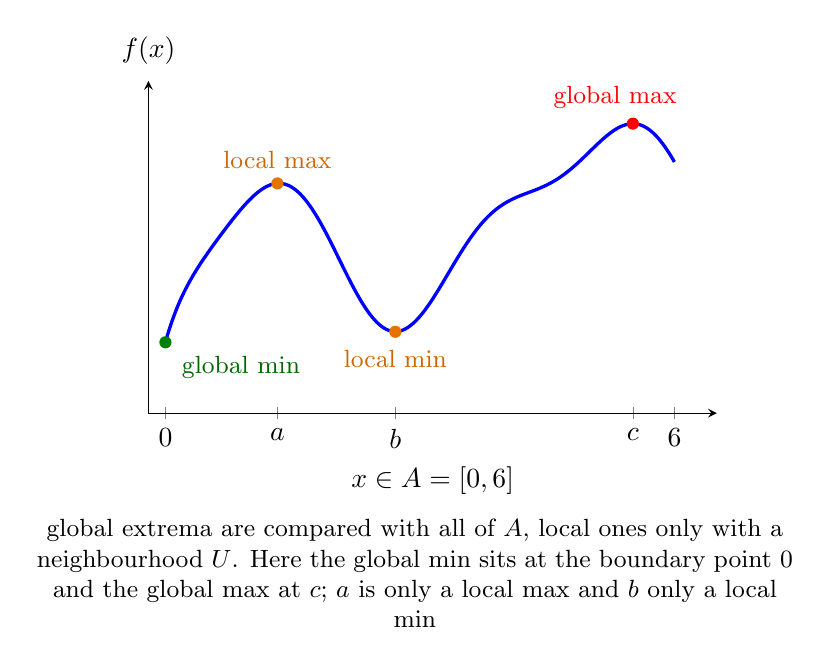
\begin{tikzpicture}
	\begin{axis}[
		axis lines=left, xmin=-0.2, xmax=6.5, ymin=-0.3, ymax=5.7,
		xtick={0,1.32,2.71,5.51,6}, xticklabels={$0$,$a$,$b$,$c$,$6$}, ytick=\empty,
		xlabel={$x\in A=[0,6]$}, ylabel={$f(x)$}, ylabel style={rotate=-90, anchor=south, at={(axis description cs:0,1.02)}},
		samples=300, smooth, width=8.8cm, height=5.8cm, clip=false
		]
		\addplot[blue, very thick, domain=0:6] {2.2+1.3*sin(deg(1.5*x+0.3))-0.5*sin(deg(3*x))+0.25*x-1.6*exp(-3*x)};
		\fill[red] (axis cs:5.51,4.93) circle (2.2pt);
		\node[red, anchor=south, font=\small] at (axis cs:5.3,5.03) {global max};
		\fill[orange!90!black] (axis cs:1.32,3.85) circle (2.2pt);
		\node[orange!80!black, anchor=south, font=\small] at (axis cs:1.32,3.95) {local max};
		\fill[orange!90!black] (axis cs:2.71,1.17) circle (2.2pt);
		\node[orange!80!black, anchor=north, font=\small] at (axis cs:2.71,1.02) {local min};
		\fill[green!50!black] (axis cs:0,0.98) circle (2.2pt);
		\node[green!40!black, anchor=north west, font=\small] at (axis cs:0.08,0.9) {global min};
	\end{axis}
	\node[anchor=north, font=\small, align=flush center, text width=9.6cm] at ([yshift=-2pt]current axis.outer south) {global extrema are compared with all of $A$, local ones only with a neighbourhood $U$. Here the global min sits at the boundary point $0$ and the global max at $c$; $a$ is only a local max and $b$ only a local min};
\end{tikzpicture}
\end{document}
